% !TeX encoding = UTF-8
% !TeX spellcheck = en_US

\chapter{Introduction}
\label{introduction}

\textit{Model-driven engineering} (MDE) is an approach to software development which focuses on the specification of software artifacts in the application domain.
It raises the abstraction level from programming to domain-specific modeling languages by the use of \textit{models} for the representation of knowledge.
The MDE approach aims for a simplification of the specification process and improvement of the communication between different people and teams working on a system (cf. \cite{MDEVoelter}, p. 13; \cite{HerringMernikWhenAndHowDevelopDSLs}).

\textit{Model transformations} \cite{SurveyOfModelTransformationApproaches} can be used to transform models into other models, \eg modifying an existing model or generating code from a model.
Other application areas are web applications \cite{ModelTransformationsWithinWebApplications}, handling XML documents \cite{KurtevXMLApplicationsWithModelTransformations}, interface design, and many others \cite{BxTransformationsCrossDisciplinePerspective}.
Because of the focus on models as primary artifacts, model transformations are a fundamental part of MDE.

\section{Graphs and Graph Transformations}
\label{graph-transformations}
Since many models can be represented as graphs (\eg UML\footnote{cp. UML 2.5 \cite{UMLSpecification}, Annex E} or XML documents), \textit{graph transformations} (GT) are a frequently used formalism to implement model transformations.
They consist of a set of \textit{graph transformation rules} of the form $L \rightarrow R$.
The left-hand side $L$ (called pattern graph) specifies the context in which the rule may be applied to a given host graph, while the right-hand side $R$ defines the elements with which the context is replaced during rule application.\footnote{Formal foundations as needed for this thesis will be introduced in Chapter \ref{fundamentals}.}

Using this declarative approach for the specification of model transformation, a rule engine can be used to find a match in the host graph conforming to the pattern graph $L$ and apply the rule.

\section{eMoflon::IBeX}
\label{emoflon-ibex}
The graph transformation tool we\footnote{Despite the use of the authorial we in this thesis, it has been written by its single author, as stated in the declaration of authorship.
The authorial we serves to increase the readability of the thesis.} shall work with in this thesis is the Eclipse-based tool \textit{eMoflon}, which is currently being reimplemented in the \textit{eMoflon::IBeX} project.\footnote{see \url{https://github.com/eMoflon/emoflon-ibex}}
Unlike the code generation based \textit{eMoflon::SDM/TiE},\footnote{see \url{https://github.com/eMoflon/emoflon-tool}. \\
	eMoflon::SDM refers to the story driven modeling part (graph transformations and control flow) of the latest eMoflon release using Enterprise Architect and code generation. \\
	eMoflon::TiE (Tool Integration Environment) allows to specify TGG rules in textual syntax. It relies on code generation and a transformation to SDMs.}
eMoflon::IBeX uses an interpreter which is completely based on incremental pattern matching.

eMoflon::TiE and eMoflon::IBeX provide a textual editor for transformation rules with syntax highlighting and checks for compliance to the meta-models specified in Ecore, the UML-like meta-modeling language of the \textit{Eclipse Modeling Framework} (EMF).
A graphical visualization of specified rules generated from the textual syntax is provided for better understandability.

While eMoflon::SDM/TiE supports both unidirectional graph transformations and bidirectional transformations between two different meta-models based on \textit{Triple Graph Grammars} (TGGs)\footnote{TGGs \cite{TGGs} are a grammar-based approach to specify a consistency relation between two models.
From the specification different operationalizations such as model generation, model synchronization, and checking the consistency of existing models can be derived.} as an underlying formalism, only the transformations with TGGs have been ported to eMoflon::IBeX (herein after referred to as \textit{eMoflon::IBeX-TGG}).
The goal of this thesis is to extend eMoflon::IBeX by unidirectional model transformations modifying a model instance by applying graph transformation rules.


\section{Running Example: She Remembered Caterpillars}
\label{running-example}
The running example used in this thesis is based on a simplified version of the game \textit{She Remembered Caterpillars}.\footnote{\url{http://caterpillar.solutions/} or  \url{http://store.steampowered.com/app/470780/She_Remembered_Caterpillars/}. The rules describe only a limited subset of the actual game.}
The use of graph transformation for this game has been suggested and applied by Zündorf et al. \cite{UsingGTforPuzzleGame}.
An example instance of this game is shown in Figure~\ref{fig:she-remembered-caterpillars-example}.\footnote{Figure~\ref{fig:she-remembered-caterpillars-example} is taken from the slides of the lecture ``Fundamentals of Model-Driven Engineering'' by Anthony Anjorin, whose examples are partly inspired by \cite{UsingGTforPuzzleGame}.}
The meta-model is shown in Figure~\ref{fig:she-remembered-caterpillars-class-diagram} as a class diagram.

\begin{figure}[h!]
	\centering
	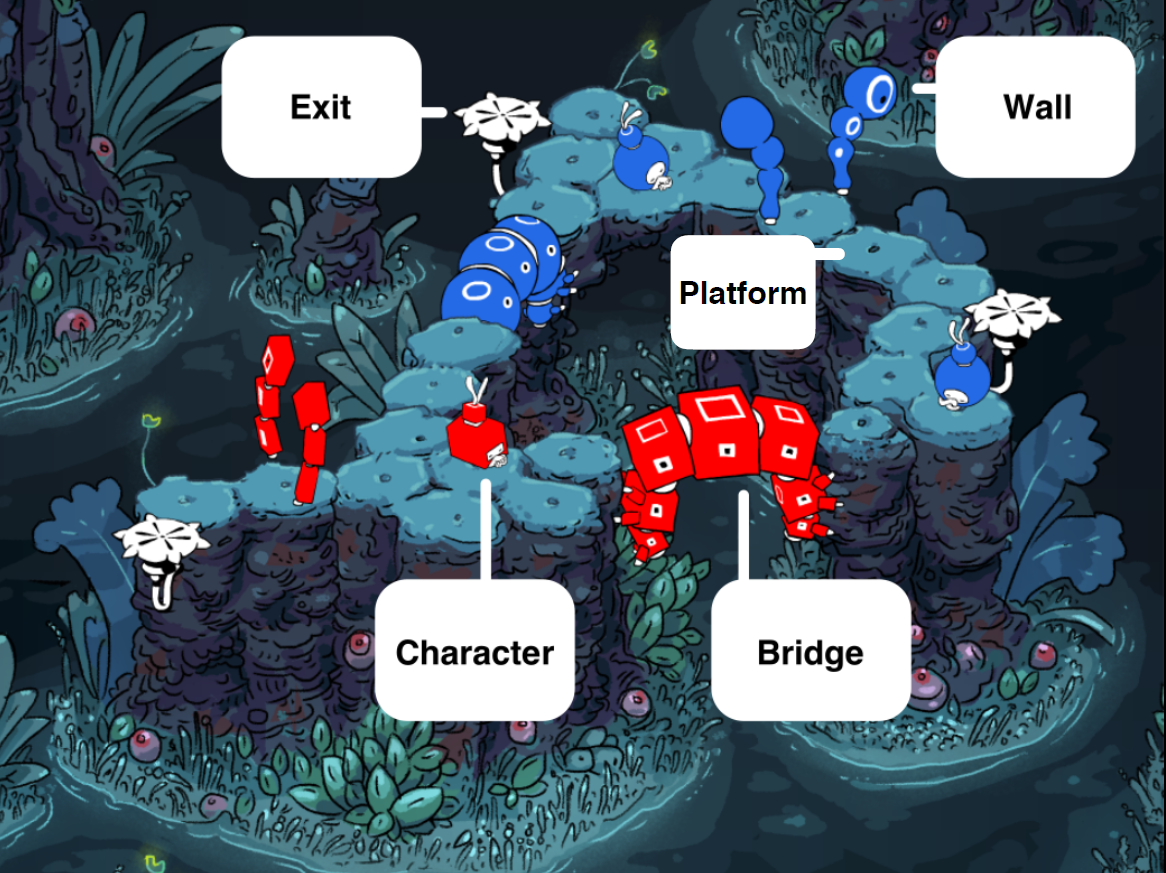
\includegraphics[width=.5\linewidth]{../common/figures/she-remembered-caterpillars-game}
	\caption{She Remembered Caterpillars Example}
	\label{fig:she-remembered-caterpillars-example}
\end{figure}

The She Remembered Caterpillars world contains simple and exit platforms which are connected to neighboring platforms.
Simple platforms can be connected via bridges and walls as well.

The goal of the game is to move all characters to exit platforms.
At the beginning, characters are placed on arbitrary platforms.
Only one character may stand on each exit platform at the end.

Characters, bridges and walls are colored blue, red or purple. 
The following rules define how characters can be moved:
\begin{enumerate}
	\item All characters can walk from their current platform to any neighboring one.
	\item Blue and red characters can cross bridges having the same color as the character and walk over walls which are not colored in the character color.
	\item Purple characters can cross any bridge, but cannot walk through any wall.
	\item If a red and a blue character stand on the same platform, they can be transformed into one purple character.
	\item A purple character can be transformed into a blue and a red character, both standing on the same platform after the transformation.
\end{enumerate} 

\begin{figure}[h!]
	\centering
		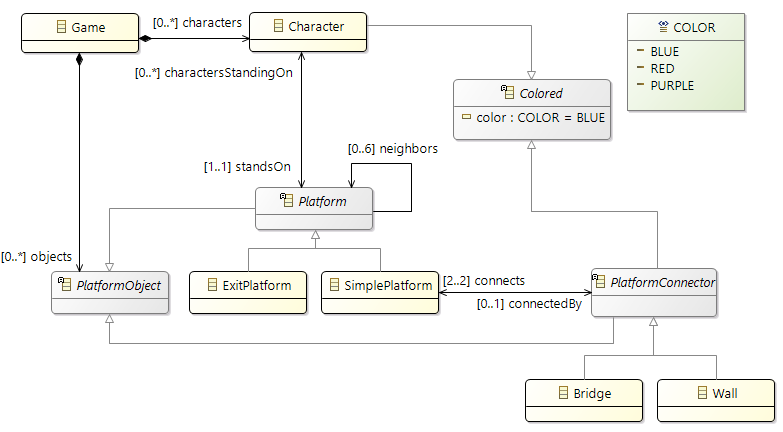
\includegraphics[width=.9\linewidth]{../common/figures/she-remembered-caterpillars-class-diagram}
	\caption{She Remembered Caterpillars Class Diagram}
	\label{fig:she-remembered-caterpillars-class-diagram}
\end{figure}

\noindent
All examples in the following chapters will use the She Remembered Caterpillars meta-model.
We will check constraints on models, create new models and write transformation rules for the different steps of the game.

\section{Contribution}
The goal of this thesis is to implement and evaluate a new tool for unidirectional graph transformations called \textit{eMoflon::IBeX-GT}, which is based on an interpreter and incremental pattern matching.
The rules can be invoked from Java code via a typed Java API generated from the textual rule specification.

eMoflon::IBeX-GT shall support simple patterns, rules, attribute assignments and conditions, pattern refinement, and application conditions.
For each of the mentioned features the main steps for the implementation are:
\begin{enumerate}
	\item the development of a textual editor for pattern and rule specifications and a graphical visualization of them,
	\item the definition of an IBeX pattern model, \ie a pattern network specification independent from a concrete pattern matching engine,
	\item the implementation of the transformation from the editor specification into the IBeX pattern model (and from the IBeX pattern model into the Democles representation),
	\item the design and the generation a typed Java API,
	\item the extension of the interpreter used for API execution,
	\item establishing a JUnit test suite to show the successful usage for a set of examples,
	\item and providing documentation for end-users.
\end{enumerate}

\noindent
As we plan to integrate the new tool into the eMoflon::IBeX toolsuite, we want to explore and exploit the potential of Democles, the underlying incremental pattern matcher used in eMoflon::IBeX-TGG already.
The following research questions shall be investigated in this thesis:
\begin{description}
	\item[RQ 1]
		Which tasks are best solved using an incremental pattern matcher?
	\item[RQ 2]
		How can a GT and TGG tool be seamlessly integrated for developers and end users?
	\item[RQ 3]
		How can we integrate graph transformations seamlessly into Java code using the power of Java 8 features such as streams?
\end{description}

\section{Structure of the Thesis}
The remainder of this thesis is organized as follows:
Chapter~\ref{fundamentals} introduces the theory on graphs, graph transformations rules and their application.
Our requirements specified in Chapter~\ref{requirements} will be evaluated for existing graph transformation tools in Chapter~\ref{related-work}.
Chapter~\ref{concept-and-implementation} deals with the transformation from the specification of patterns in the editor into pattern networks.
The generation of a typed API and the invocation from Java code via the API is presented in Chapter~\ref{api}.
Chapter~\ref{evaluation} evaluates the new tool with respect to the requirements, correctness, and performance.
Finally, we discuss future work in Chapter~\ref{future-work}.
